\documentclass[11pt,a4paper]{article}

% -------------------------------------------------
% ENCODAGE / LANGUE
% -------------------------------------------------
\usepackage[utf8]{inputenc}
\usepackage[T1]{fontenc}
\usepackage[french]{babel}

% -------------------------------------------------
% MISE EN PAGE
% -------------------------------------------------
\usepackage[a4paper,margin=2.5cm]{geometry}
\usepackage{setspace}
\usepackage{parskip}

% -------------------------------------------------
% MATHS / IMAGES / TABLEAUX
% -------------------------------------------------
\usepackage{amsmath,amssymb}
\usepackage{graphicx}
\usepackage{booktabs}
\usepackage{array}
\usepackage{float}

% -------------------------------------------------
% LIENS
% -------------------------------------------------
\usepackage[colorlinks=true,linkcolor=black,urlcolor=blue,citecolor=black]{hyperref}

% -------------------------------------------------
% CODE (optionnel)
% -------------------------------------------------
\usepackage{xcolor}
\usepackage{listings}
\renewcommand{\lstlistingname}{Code}

\definecolor{backcolour}{rgb}{0.95,0.95,0.95}
\definecolor{codegreen}{rgb}{0,0.5,0}
\definecolor{codegray}{rgb}{0.4,0.4,0.4}

\lstdefinestyle{mystyle}{
    backgroundcolor=\color{backcolour},
    commentstyle=\color{codegreen},
    numberstyle=\tiny\color{codegray},
    basicstyle=\ttfamily\small,
    breaklines=true,
    numbers=left,
    numbersep=5pt,
    showstringspaces=false
}

\lstset{
    basicstyle=\ttfamily\scriptsize,
    backgroundcolor=\color{gray!10},
    frame=single,
    breaklines=true,
    captionpos=b
}

\lstset{
  literate=
  {á}{{\'a}}1 {é}{{\'e}}1 {í}{{\'i}}1 {ó}{{\'o}}1 {ú}{{\'u}}1
  {Á}{{\'A}}1 {É}{{\'E}}1 {Í}{{\'I}}1 {Ó}{{\'O}}1 {Ú}{{\'U}}1
  {à}{{\`a}}1 {è}{{\`e}}1 {ì}{{\`i}}1 {ò}{{\`o}}1 {ù}{{\`u}}1
  {À}{{\`A}}1 {È}{{\'E}}1 {Ì}{{\`I}}1 {Ò}{{\`O}}1 {Ù}{{\`U}}1
  {ä}{{\"a}}1 {ë}{{\"e}}1 {ï}{{\"i}}1 {ö}{{\"o}}1 {ü}{{\"u}}1
  {Ä}{{\"A}}1 {Ë}{{\"E}}1 {Ï}{{\"I}}1 {Ö}{{\"O}}1 {Ü}{{\"U}}1
  {â}{{\^a}}1 {ê}{{\^e}}1 {î}{{\^i}}1 {ô}{{\^o}}1 {û}{{\^u}}1
  {Â}{{\^A}}1 {Ê}{{\^E}}1 {Î}{{\^I}}1 {Ô}{{\^O}}1 {Û}{{\^U}}1
  {œ}{{\oe}}1 {Œ}{{\OE}}1 {æ}{{\ae}}1 {Æ}{{\AE}}1
  {ç}{{\c{c}}}1 {Ç}{{\c{C}}}1 {¿}{{\textquestiondown}}1 {¡}{{\textexclamdown}}1
}

% -------------------------------------------------
% TITLE
% -------------------------------------------------
\title{\textbf{RCP103 -- Rapport de TP}\\TP02 - Création d'un simulateur de file d'attente\\Partie 1}
\author{BOURDAYA Amina, BOUTY Gabriel, CLERC Julien}
\date{\today}

% -------------------------------------------------
% DOCUMENT
% -------------------------------------------------
\begin{document}

\maketitle

\bigskip
\bigskip

\begin{abstract}
    Ce TP à pour objectif de créer un programme permettant de simuler un système simple de type Client(s)/Server(s) asynchrones.
    Ce premier document présente l'inititalisation du projet, la schématisation du simulateur, et la description de la réalisation des premiers composants.
\end{abstract}

\bigskip
\bigskip

% -------------------------------------------------
\section{Description du système simulé}

Comme évoqué en introduction, ce rapport présente la première phase de réalisation d'un simple simulateur Client(s)/Server(s):

Un ensemble de $M$ clients ($M >= 1$), envoient des messages à $N$ serveurs ($N >= 1$). Un portail sert d'intermédiaire entre clients et serveurs. Compte tenu que les serveurs ne peuvent traiter qu'un message à la fois, le portail permet de temporiser les messages en attente de traitement dans un tampon de taille fixe $K$.

\begin{figure}[H]
    \centering
    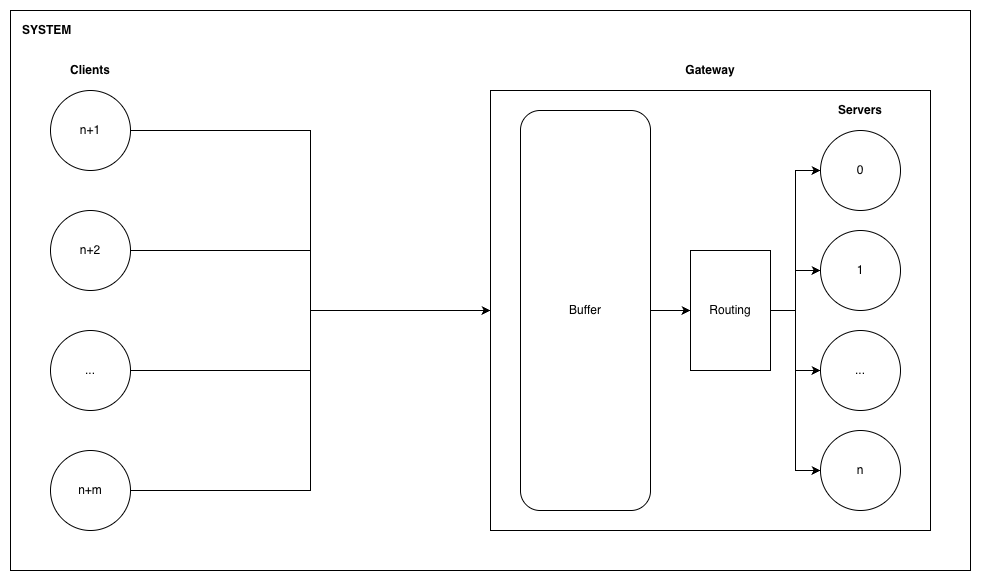
\includegraphics[width=0.80\textwidth]{../images/system.png}
    \caption{Schéma du système simulé}
\end{figure}

Dans ce simulateur, les envois de messages suivent un processus de Poisson: le taux d'envois est constant dans le temps, les temps entre deux envois consécutifs suivent une distribution exponentielle. De même, le temps de service suit une loi exponentielle.

Dans un premier temps, nous limiterons notre simulateur à un seul serveur, nous pourrons donc simuler un processus de file d'attente de type M/M/1/K:

\begin{itemize}
    \item M: Arrivées selon un processus de Poisson (Markovien).
    \item M: Temps de service selon une distribution exponentielle (Markovien).
    \item 1: Nombres de serveurs (ici, 1).
    \item K: Capacité du système (ici, la taille du tampon du portail de capacité K).
\end{itemize}

\bigskip

\bigskip

% -------------------------------------------------
\section{Architecture du simulateur}
\subsection{Architecture initiale}
\bigskip
\subsection{Organisation du code source}
\bigskip

\bigskip

% -------------------------------------------------
\section{Créations des premières classes}
\subsection{Les données: class Message et class Event}
\bigskip
\subsection{L'ordonnanceur: class Scheduler}
\bigskip
\subsection{Les fonctions de logs: functions Trace}
\bigskip
\subsection{Le cœur du système: class Engine}
\bigskip
\subsection{Le point d'entrée: function main}
\bigskip

\bigskip

% -------------------------------------------------
\section{Tests des premières classes}
\subsection{Le système de test: Pytest}
\bigskip
\subsection{Présentation des tests rédigés}
\bigskip
\subsection{Exécution des tests}
\bigskip

\bigskip


% -------------------------------------------------
\section{Conclusion}


\end{document}
